%Do not touch first page!
\section{Formale Sprachen}
    \begin{itemize}
        \item Was ist die Theorie Formaler Sprachen?
        \begin{itemize}
            \item schlecht definierter Begriff!
        \end{itemize}
        \item Sei $\Sigma$ eine \emph{endliche} Menge, die wir Alphabet nennen
        \item $\Sigma^*$ ist die Menge der \emph{endlichen} Sequenzen von $\Sigma$-Elementen
        \item Eine (formale) Sprache ist die Teilmenge von $\Sigma^*$
        \item Es gibt $2^{|\Sigma^*|}>|\mathds{N}|$ Sprachen, uns interessieren nur abzählbar viele davon.
        \item Wir stellen Sprachen durch endliche Beschreibungen dar
            \begin{itemize}
                \item Grammatik
                \item Automaten (Endlich, Keller, Turingmaschine,\dots)
                \item Logik
                \item Algebra
                \item Schaltkreise
                \item Ausdrücke
                \item \dots
            \end{itemize}
    \end{itemize}\vspace*{-2cm}\hspace*{6cm}\vspace*{-7cm} %!!!
    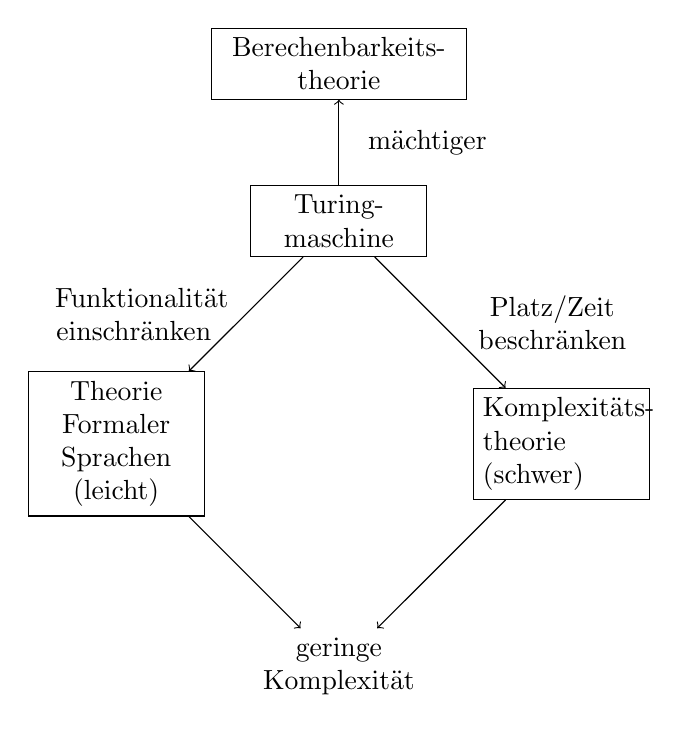
\begin{tikzpicture}[node distance=4cm,->]
        \node[rectangle,align=center,draw,text width=2cm] (TM) {Turing\-maschine};
        \node[rectangle,align=center,draw,text width=3cm] (BT) [above of=TM,yshift=-2cm] {Berechenbarkeits-\\theorie};
        \node[rectangle,align=center,draw,text width=2cm] (TFS) [below left of=TM] {Theorie Formaler\\ Sprachen (\qq{leicht})};
        \node[rectangle,draw,text width=2cm] (K) [below right of=TM] {Komplexitäts\-theorie \\(\qq{schwer})};
        \node (l) [below right of=TFS,align=center,text width=2cm] {geringe Komplexität};
        \path (TM) edge node[right,align=center,text width=2cm]{mächtiger} (BT)
            (TM) edge node[xshift=.3cm,right,align=center,text width=2cm]{Platz/Zeit\\beschränken} (K)
            (TM) edge node[xshift=-.3cm,left,align=center,text width=2cm]{\qq{Funktionalität} einschränken} (TFS)
            (TFS) edge (l)
            (K) edge (l);
    \end{tikzpicture}\newpage
\section{Wiederholung Theoretische Informatik}
    \subsection{Chomsky-Hierarchie}
        \begin{itemize}
            \item[] Alle Sprachen
                \begin{itemize}
                    \item[$\supset$] Typ 0 (Turingmaschine)
                    \begin{itemize}
                        \item[$\supset$] Typ 1 (kontextsensitiv) ($\mathcal{O}(n)$ Platz)
                        \begin{itemize}
                            \item[$\supset$] Typ 2 (kontextfrei) (Kellerautomat)
                            \subitem$\supset$ Typ 3 (regulär) (endlicher Automat)
                        \end{itemize}
                    \end{itemize}
                \end{itemize}
        \end{itemize}
    \subsection{Berechenbarkeit}
        \begin{itemize}
            \item Church-Turing-These
            \begin{itemize}
                \item Sprache entscheidbar $\Leftrightarrow$ charakteristische Funktion berechenbar ($\Rightarrow$ Wortproblem, andere lassen sich darauf abbilden)
            \end{itemize}
            \item Reduktion: $A\le_m B :\Leftrightarrow \left(\exists f: x\in A\Leftrightarrow f(x)\in B\right)$ (many-one Reduktion)
            \item Reduktion (Turing): $A\le_T B:\Leftrightarrow\exists TM$ mit Orakel $B$, die $A$ erkennt.
        \end{itemize}
    \subsection{Komplexitätstheorie}
        \begin{itemize}
            \item L ist C-schwer $:\Leftrightarrow\forall X\in C: X\le L$
            \item L ist C-vollständig $:\Leftrightarrow$ L ist C-schwer und L$\in$ C
        \end{itemize}
        \begin{figure}
            \centering
            \label{fig:complexity}
            \begin{tikzpicture}
                [node distance=0.1\textheight]
                \node (PSP) {PSPACE};
                \node (NP) [below left of=PSP] {NP};
                \node (NSP) [below right of=PSP] {NSPACE(n)=Typ 1};
                \node (P) [below of=NP] {P};
                \node (NL) [below right of=P] {NL$\supseteq$ Typ 2};
                \node (DSP) [below of=NSP] {DSPACE(n)};
                \node (L) [below of=NL] {L};
                \node (NC) [below of=L] {NC$^1\supseteq$ Typ 3};
                \node (TC) [below of=NC] {TC$^0$};
                \node (ACC) [below of=TC] {ACC$^0$};
                \node (AC) [below of=ACC] {AC$^0$};
                \path (PSP) edge (NP)
                    (PSP) edge (NSP)
                    (NP) edge (P)
                    (NSP) edge (DSP)
                    (P) edge (NL)
                    (DSP) edge (NL)
                    (NL) edge (L)
                    (L) edge (NC)
                    (NC) edge (TC)
                    (TC) edge (ACC)
                    (ACC) edge (AC);
                \draw[decorate, decoration={brace, amplitude=10pt}] (3,.2) -- node[right,xshift=10pt]{TM} (3,-7.4) ;
                \draw[decorate, decoration={brace, amplitude=10pt}] (3,-7.4) -- node[right,xshift=10pt]{Schaltkreis} (3,-14.3) ;
                \draw[dashed] (-5,-7.4) -- (5,-7.4);
            \end{tikzpicture}
            \caption{Komplexitätsklassen}
        \end{figure}
    \subsection{Theorie formaler Sprachen}
        \subsubsection{Reguläre Sprachen} % (fold)
        \label{ssub:intro-reg}
            \begin{itemize}
                \item REG = Typ3-Grammatik = DEA = NEA = reguläre Ausdrücke = endliche Monoide
                \item NEA $\rightarrow$ DEA: Potenzmengenkostruktion
                \item DEA: Minimalautomat, vgl. Myhill-Nerode
                \item Abschlüsse: Komplement, Schnitt, Vereinigung, Konkatenation, Stern, Homomorphismen, inverse Homomorphismen, Quotienten, \dots
                \item Entscheidbarkeit: Wort, Leerheit, Äquivalenz, Endlichkeit
                \item Tradeoff: Abschluss und Entscheidbarkeit vs. Ausdrucksstärke
                \item Pumping Lemma
            \end{itemize}
        % subsubsection intro-reg (end)
        \subsubsection{Kontextfreie Sprachen} % (fold)
        \label{ssub:intro-kf}
            \begin{itemize}
                \item Kellerautomaten = Typ 2-Grammatiken
                \item Wortproblem: CYK $\mathcal{O}(n^3)$ Laufzeit
                \item CNF: $A\rightarrow BC,\ A\rightarrow a$ ($\Rightarrow$ binärer Ableitungsbaum)
                \item Abschlüsse: Vereinigung, Konkatenation, Stern
                \item nicht abgeschlossen unter: Komplement, Schnitt
                \item Entscheidbarkeit: Wortproblem, Leerheit
                \item nicht entscheidbar: Äquivalenzproblem
                \item Pumping Lemma
            \end{itemize}
        % subsubsection intro-kf (end)
\section{Wiederholung Formale Sprachen I}
    \subsection{Algebra} % (fold)
    \label{sub:intro-algebra}
        \begin{itemize}
            \item Homomorphismus: $\varphi(w_1w_2)=\varphi(w_1)\varphi(w_2)$
            \item Monoid: abgeschlossen, assoziativ und neutrales Element existiert
            \item $\varphi : \Sigma^* \rightarrow M,\ X\subseteq M$, dann ist $\varphi^{-1}(X)$ eine Sprache
            \subitem oder: $L\subseteq \Sigma^*$ wird von M erkannt $\Leftrightarrow L=\varphi^{-1}\left(\varphi\left(L\right)\right)$
            \item L regulär $\Leftrightarrow$ L wird von endlichem Monoid erkannt.
        \end{itemize}
    % subsection intro-algebra (end)
    \subsection{Logik} % (fold)
    \label{sub:intro-logik}
        \begin{itemize}
            \item Beispiel:
            \begin{itemize}
                \item $\exists x\forall y: y\le x\wedge Q_a(x) \in FO[\le]$ (\qq{Wort endet auf a})
                \item $\exists X$\dots (monadische Logik 2. Ordnung (MSO))
            \end{itemize}
            \item später mehr
        \end{itemize}
    % subsection intro-logik (end)
